\begin{abstract}
This paper presents a study on the application of machine learning and deep learning techniques for the classification and segmentation of breast tumour ultrasound images. The main objective of the study is to classify tumours into three classes-categories: i)normal, ii)benign, and iii)malignant, and to identify cancerous regions within the images. The methodology that was followed involves training and evaluating models using both traditional machine learning and deep learning algorithms. Furthermore, explainability techniques are applied to deep learning cases, in order to gain insights into the model's decision-making process. The results demonstrate the effectiveness of deep learning models in achieving high classification accuracy and accurate tumour segmentation. The findings contribute to the field of medical image analysis and provide a foundation for further research and development of automated breast tumour diagnosis systems.
\end{abstract}

\section{Introduction}
Breast cancer is a prevalent disease affecting millions of women worldwide, emphasizing the importance of early detection and accurate diagnosis of breast tumours for effective treatment and improved patient outcomes. Medical imaging, particularly ultrasound imaging, plays a crucial role in diagnosing breast tumours. However, interpreting ultrasound images poses challenges due to the complexity and variability of tumour appearances.

In this paper, we investigate the application of machine learning and deep learning techniques for classifying and segmenting breast tumour ultrasound images. The classification task focuses on categorizing tumours into three classes: normal, benign, and malignant, aiding radiologists in the initial assessment of tumour malignancy. Simultaneously, the segmentation task aims to identify cancerous regions within the images, regardless of their specific malignant characteristics, facilitating targeted analysis and treatment planning.

To address these challenges comprehensively, we adopt a multi-faceted approach. Initially, we employ traditional machine learning algorithms, such as support vector machines (SVM) and random forests, to classify breast tumours based on handcrafted features. Subsequently, we explore the potential of deep learning models, specifically convolutional neural networks (CNNs), for both classification and segmentation tasks. These deep learning models leverage end-to-end feature learning, automatically extracting meaningful features from ultrasound images.

To ensure transparency and interpretability of the deep learning models, we incorporate explainability techniques, such as Grad-CAM (Gradient-weighted Class Activation Mapping), which visualize and provide insights into the regions of interest contributing to the model's decision-making process. This integration of classification, segmentation, and explainability offers a comprehensive analysis of breast tumour ultrasound images.

Our contributions encompass the development and evaluation of machine learning and deep learning models for breast tumour classification and segmentation. The results demonstrate the superior performance of deep learning models in terms of accuracy and provide valuable insights into model interpretability. This research lays the groundwork for automated breast tumour diagnosis systems, assisting healthcare professionals in the accurate and timely detection of breast cancer.

The dataset used in this study is referenced as \cite{dataset}, which provides a diverse collection of breast ultrasound images for training and evaluation purposes.

Please note that the baseline accuracy for this task is $56.03\%$, highlighting the significance of our proposed techniques in achieving substantial improvements in breast tumour classification and segmentation accuracy.

\section{Image Classification Using Machine Learning Algorithms}

\subsection{Description}
In this section, we employ traditional machine learning techniques to classify the provided breast ultrasounds into three classes: i) normal, ii) benign, and iii) malignant. The section covers the key steps involved in this analysis, including data preprocessing, feature extraction from each image, and training and evaluating models such as Support Vector Machines (SVM) and Random Forest. The results generated by our pipeline are presented at the end of this section.

\subsection{Data Preprocessing}
Given that our input consisted of pure grayscale images, data preprocessing was a straightforward task. Our main objective was to resize all the images to a consistent dimension, as the ultrasound images varied in size. We opted to resize the images to (256, 256) dimensions, ensuring data uniformity across the dataset. Additionally, we partitioned our dataset into training and test sets. The training dataset comprises $80 \%$ of the initial dataset, while the remaining $20 \%$ is allocated to the test dataset. This division ensures that we have a dedicated portion of the data for model training and evaluation, respectively. We did not utilize a separate validation dataset in our approach. Instead, we employed k-fold cross-validation for model evaluation. This technique involves dividing the training dataset into k subsets or folds and iteratively training and validating the model on different combinations of these folds. 

\subsection{Feature Extraction}
The crucial aspect of image classification using traditional machine learning techniques is the selection of appropriate feature extraction methodologies. In our study, we utilized four distinct algorithms for each image, which we will now briefly describe:
\begin{itemize}
\item \textbf{HOG (Histogram of Oriented Gradients) Features:} The Histogram of Oriented Gradients (HOG) algorithm captures the distribution of gradient orientations in an image. It achieves this by dividing the image into cells and calculating the gradient magnitudes and orientations for each cell. These values are then used to construct a histogram representing the distribution of gradient orientations. HOG features are particularly effective in capturing shape and edge information within the image.
\item \textbf{Haralick Features:} Haralick Features are a type of texture-based features commonly used in image analysis. They are derived from the gray-level co-occurrence matrix (GLCM), which captures the statistical relationships between pairs of pixels in an image. Haralick features provide quantitative measures of various texture properties, including contrast, entropy, energy, and homogeneity. These features are useful for characterizing the texture patterns present in the image.
\item \textbf{GLSZM (Gray-Level Size Zone Matrix) Features:} GLSZM features are used to characterize the size and intensity distribution of connected regions or zones in an image. The algorithm calculates a matrix that represents the number of occurrences of different combinations of gray levels and zone sizes. GLSZM features provide insights into the heterogeneity and spatial distribution of intensity levels within an image.
\item \textbf{LBP (Local Binary Patterns) Features:} LBP features capture texture patterns based on the frequency of different binary codes in the image. LBP is commonly used for texture classification and analysis.
\end{itemize}
After applying the mentioned algorithms, we obtain 76 features for each image, which will serve as inputs to our machine learning algorithms. It is worth noting that the HOG algorithm generates over 3000 features per image. To handle this high-dimensional feature space, we applied Principal Component Analysis (PCA) and retained only the 30 most significant features. This dimensionality reduction technique allows us to reduce the computational complexity while preserving the most informative features.
\subsection{Models - Results}
Multiple classifiers have been evaluated to identify the most suitable one for our task. Throughout the training process, we experimented with the following classifiers:
\begin{itemize}
\item Linear SVM
\item Gaussian RBF SVM kernel
\item Polynomial SVM
\item Random Forest
\item Ada Boost
\end{itemize}
The training accuracy results for each classifier are presented in the following Table \ref{Table - ML_Classification Training accuracy results for each of the 5 classifiers that have been tested}
\begin{table}[H]
\centering
\begin{tabular}{cc}
\textbf{Classifier}     & \textbf{Accuracy} \\
Linear SVM              & 0.713             \\
Gaussian RBF SVM kernel & 0.67              \\
Polynomial SVM          & 0.695             \\
Random Forest           & 0.699             \\
Ada Boost               & 0.622            
\end{tabular}
\caption{Training accuracy results for each of the five classifiers that were tested during the training phase.}
\label{Table - ML_Classification Training accuracy results for each of the 5 classifiers that have been tested}
\end{table}
We performed hyperparameter tuning for the four models, excluding Ada Boost due to its low accuracy. After the tuning process, we selected the three most accurate models, namely Polynomial SVM, Linear SVM, and Random Forest. Our final model is a voting classifier that combines the predictions of the three trained models. In the following Table \ref{Table - ML_Classification Test accuracy-precision-recall-f1 results for voting classifier}, we present the results obtained from the voting classifier when applied to test set. It showcases the accuracy, precision, recall, and F1-score of the classifier for each class.
\begin{table}[H]
\centering
\begin{tabular}{cc}
Accuracy  & 0.7308                 \\
Precision & 0.6428, 0.7212, 0.7895 \\
Recall    & 0.3214, 0.9146, 0.6521 \\
F1 score  & 0.4286, 0.8064, 0.7143
\end{tabular}
\caption{The metrics for the test set using the voting classifier that was trained. Precision, Recall, and F1 score are provided for each class separately, with the classes being normal, benign, and malignant.}
\label{Table - ML_Classification Test accuracy-precision-recall-f1 results for voting classifier}
\end{table}

The performance of the final machine learning model was assessed using various evaluation metrics to measure its accuracy and class-specific performance. The overall accuracy of the model was determined to be $73.08\%$. Precision, which evaluates the proportion of correctly predicted instances among the predicted ones, varied across different classes. For the "normal" class, the precision was $64.28\%$, indicating that approximately $64.28\%$ of the predicted "normal" instances were accurate. The "benign" class exhibited a precision of $72.12\%$, suggesting a relatively higher accuracy in identifying "benign" instances. Similarly, the "malignant" class demonstrated a precision of $78.95\%$, signifying a reasonably high accuracy in classifying "malignant" instances.

Recall, also known as sensitivity, measures the proportion of correctly predicted instances among the actual instances of a class. The recall values varied across classes, with the "normal" class displaying a recall of $32.14\%$, indicating that only around $32.14\%$ of the actual "normal" instances were correctly identified. Conversely, the "benign" class showed a recall of $91.46\%$, reflecting a high rate of accurate identification for "benign" instances. The "malignant" class had a recall of $65.21\%$, indicating a moderate level of accuracy in identifying "malignant" instances.

The F1 score, which harmoniously combines precision and recall, offers a balanced measure of the model's performance. The F1 scores for the different classes were $42.86\%$ for "normal," $80.64\%$ for "benign," and $71.43\%$ for "malignant." These scores provide an overall assessment of the model's ability to correctly classify instances for each class and account for both precision and recall.

In summary, the final model achieved an overall accuracy of $73.08\%$ and demonstrated varying levels of precision, recall, and F1 score for each class. The higher precision and recall values for the "benign" class indicate successful identification of "benign" instances, while the performance for the "normal" and "malignant" classes showed room for improvement. These results shed light on the model's strengths and limitations in classifying breast tumour ultrasound images and offer valuable insights into its overall performance.

We also provide the confusion matrix of our problem in Figure \ref{Figure - ML_Classification Confusion matrix}.
\begin{figure}
  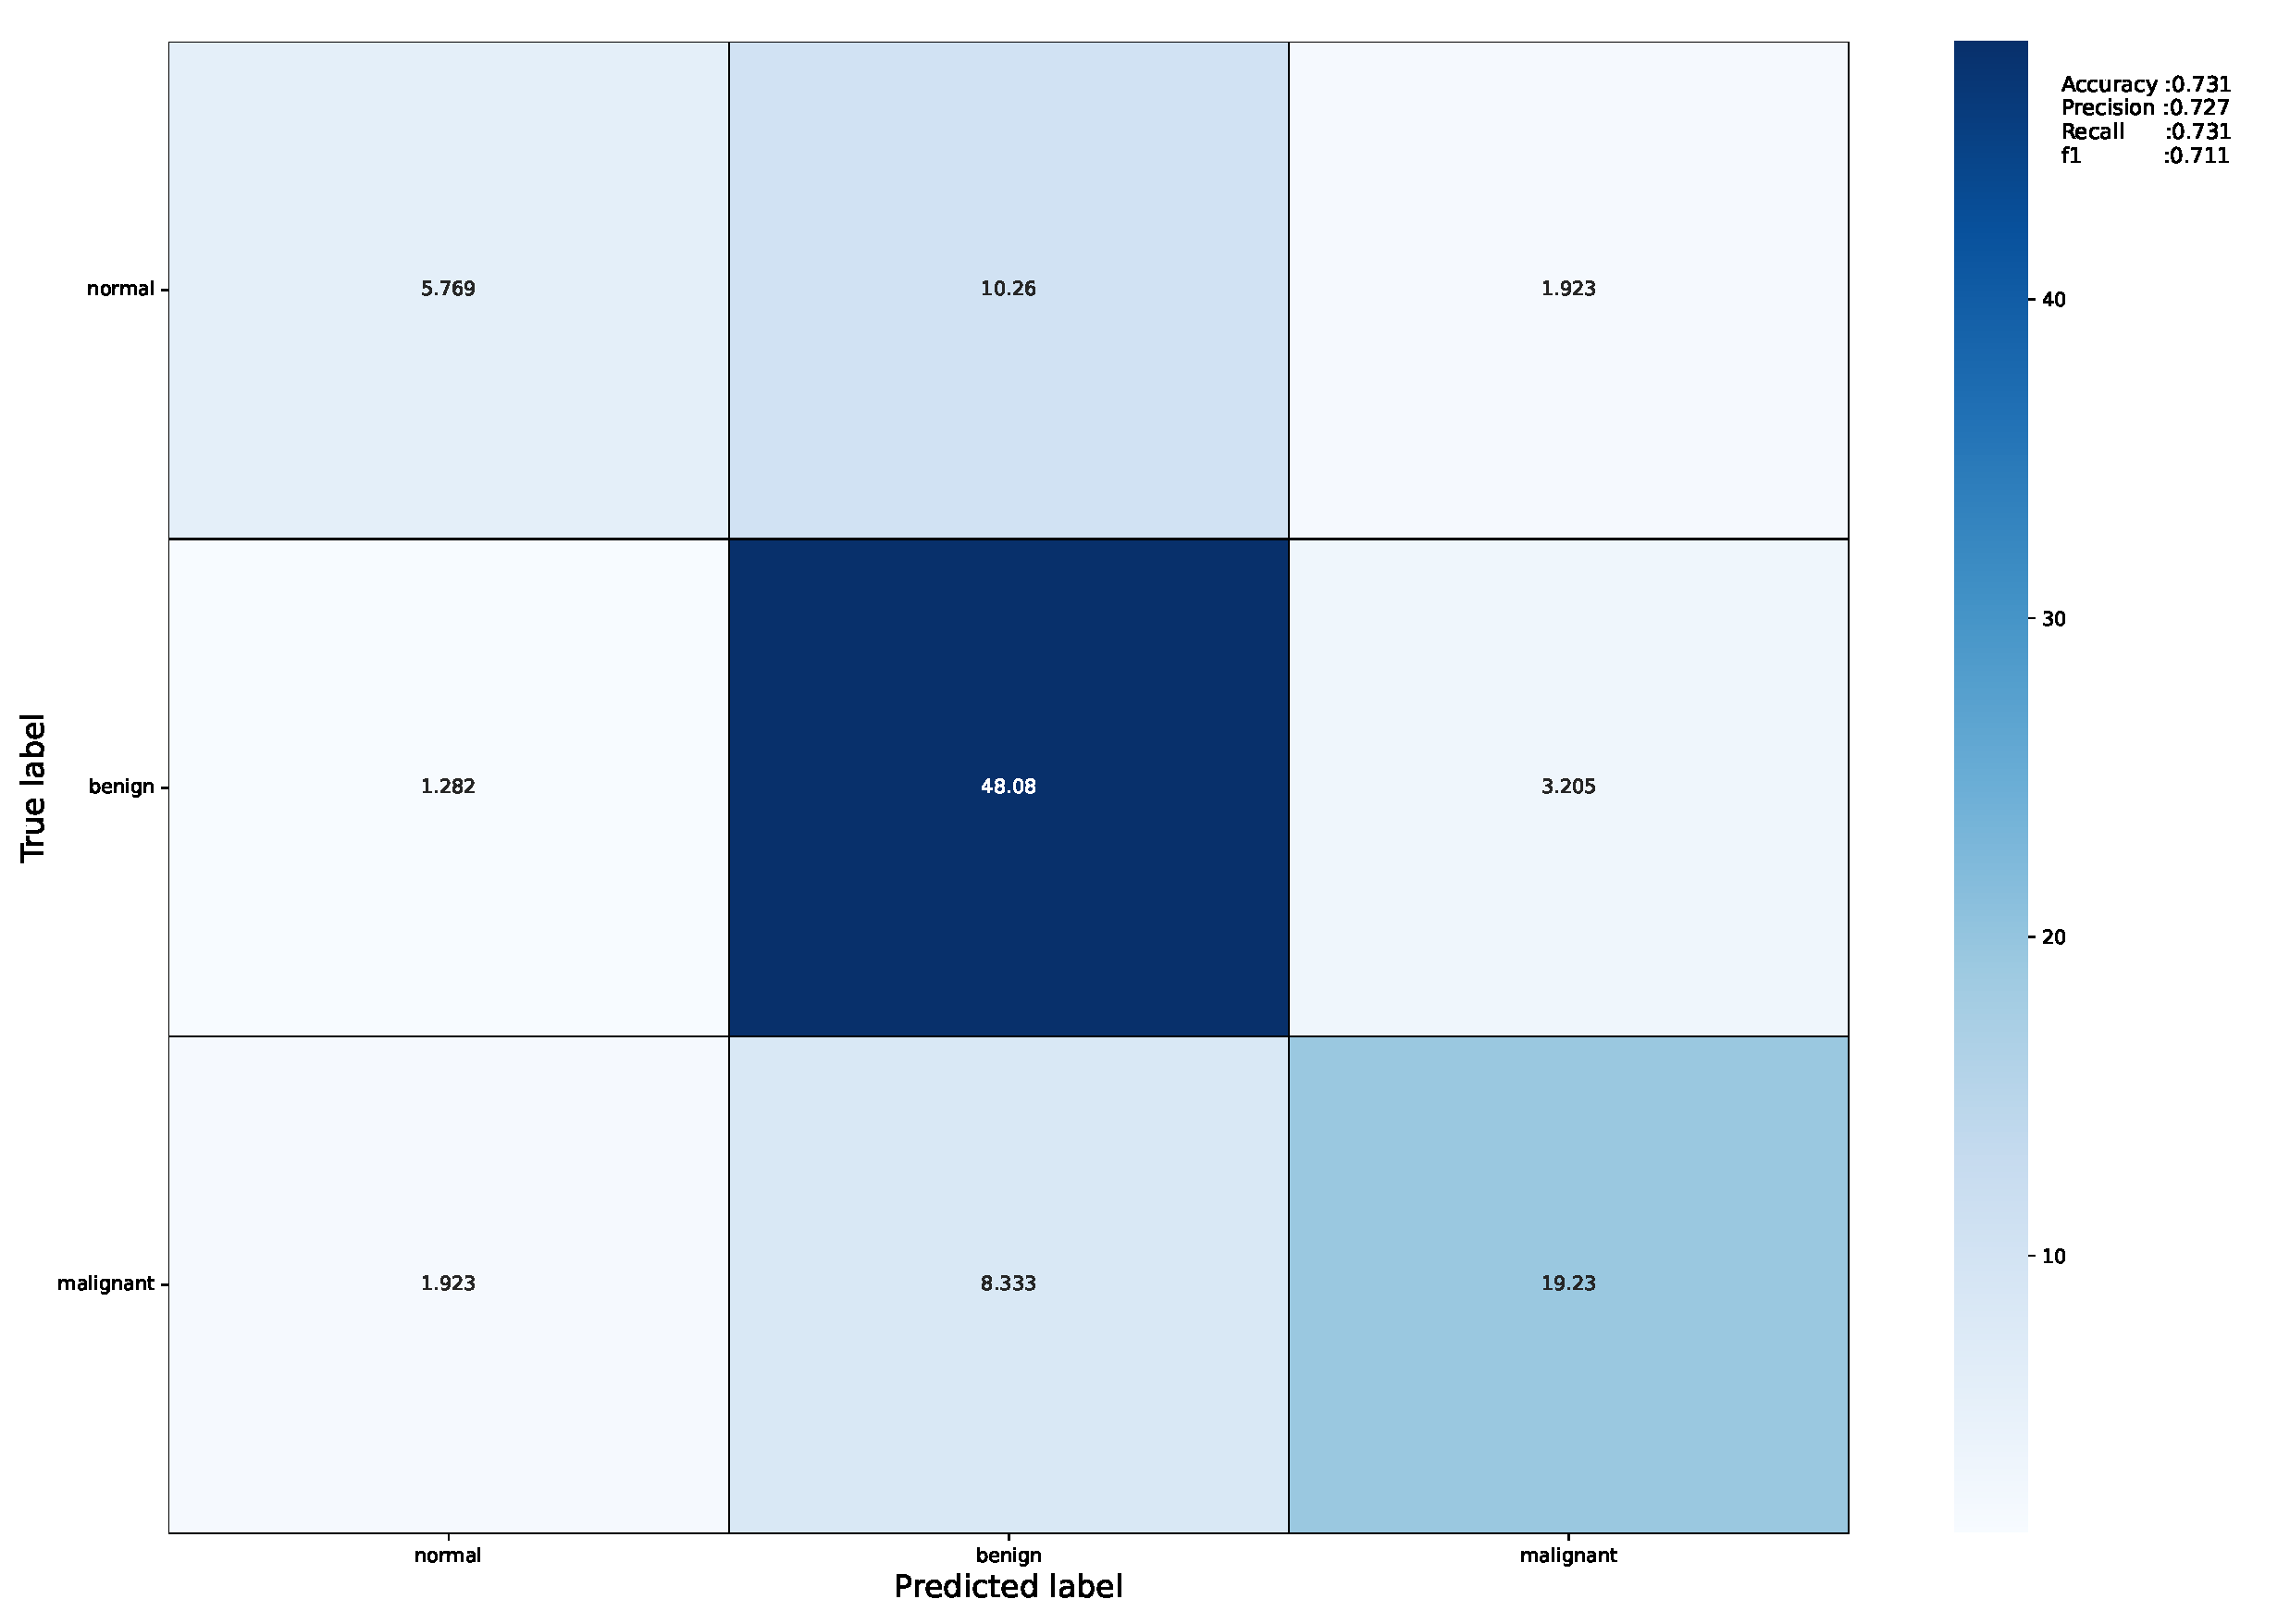
\includegraphics[width=\linewidth]{Figures/Confusion_Matrix_ML_Classification.pdf}
  \caption{Confusion matrix of traditional Machine Learning Classification task.}
  \label{Figure - ML_Classification Confusion matrix}
\end{figure}

The baseline accuracy for this task, which represents the performance of a simple or random model, was $56.03\%$.

%%%%%%%%%%%%%%%%%%%%%%%%%%%%%%%%%%%%%%%%%%%%%%%%%%%%%%%%%%%%%%%%%%%%%%%%%%%
%%%%%%%%%%%%%%%%%%%%%%%%%%%%%%%%%%%%%%%%%%%%%%%%%%%%%%%%%%%%%%%%%%%%%%%%%%%
%%%%%%%%%%%%%%%%%%%%%%%%%%%%%%%%%%%%%%%%%%%%%%%%%%%%%%%%%%%%%%%%%%%%%%%%%%%
%%%%%%%%%%%%%%%%%%%%%%%%%%%%%%%%%%%%%%%%%%%%%%%%%%%%%%%%%%%%%%%%%%%%%%%%%%%
%%%%%%%%%%%%%%%%%%%%%%%%%%%%%%%%%%%%%%%%%%%%%%%%%%%%%%%%%%%%%%%%%%%%%%%%%%%
%%%%%%%%%%%%%%%%%%%%%%%%%%%%%%%%%%%%%%%%%%%%%%%%%%%%%%%%%%%%%%%%%%%%%%%%%%%
%%%%%%%%%%%%%%%%%%%%%%%%%%%%%%%%%%%%%%%%%%%%%%%%%%%%%%%%%%%%%%%%%%%%%%%%%%%
%%%%%%%%%%%%%%%%%%%%%%%%%%%%%%%%%%%%%%%%%%%%%%%%%%%%%%%%%%%%%%%%%%%%%%%%%%%

\section{Image Segmentation Using Machine Learning Algorithms}

\subsection{Description}
In this section, we employ traditional machine learning techniques for image segmentation of the provided breast ultrasound images. The approach involves preprocessing the images, extracting features from each pixel, and evaluating the results using models like Support Vector Machines (SVM) and Random Forest.

\subsection{Data Preprocessing}
For this task, we employed a similar methodology for data preprocessing due to the varying sizes of our images. To ensure data uniformity across the dataset, we resized the images to dimensions of (128, 128). This decision was based on considerations of computational time and RAM memory required for training our models. The reduction in dimensionality allowed us to handle the massive amount of input data more efficiently.

Unlike our previous approach of extracting features for each image, we now focused on extracting features for each pixel within the images. This significantly increased the volume of input data. Previously, we processed approximately 800 images, whereas now we had to process 128 x 128 x 800 = 13,107,200 pixels. Considering that each pixel required multiple features, the scale of this task became challenging.

To simplify the process, we decided to work with a smaller subset of our dataset, utilizing only 50 images. The same preprocessing steps were applied to both the ultrasound images and their corresponding masks. The masks provided us with labels for each pixel, distinguishing between tumour and non-tumour regions. Consequently, our task transformed into a binary classification problem, where the objective was to determine whether each pixel was cancerous or not.

To enhance the accuracy of our training procedure, we implemented a cropping technique for the training images, focusing on the tumour area. The objective was to create a dataset with a baseline accuracy of approximately $50\%$. This decision was motivated by the observation that the boundary pixels in ultrasound images tend to become progressively darker. This phenomenon caused our algorithm to misinterpret these pixels as cancerous, leading to incorrect results. Thus, it became evident that this tool may not be suitable for raw ultrasound images but rather as a tool used when we have a specific area of suspicion for cancer.

\subsection{Feature Extraction}
As mentioned earlier, in our current approach, we generate features for each pixel of the image. In addition to Haralick features, we incorporate LBP (Local Binary Patterns) features and intensity-based features such as mean, skew, kurtosis, and entropy. To compute these per-pixel features, we utilize a 5x5 patch centered around each pixel, enabling us to calculate these values effectively. Due to increasing computational time, we limited the number of features to 22 per pixel, striking a balance between computational efficiency and feature richness.

\subsection{Models - Results}
We applied a similar pipeline to the image classification task, with the exception that we did not perform hyperparameter tuning due to computational limitations. Therefore, we trained the following classifiers without fine-tuning their hyperparameters:
\begin{itemize}
\item Linear SVM
\item Polynomial SVM
\item Random Forest
\item Ada Boost
\end{itemize}
The training accuracy results for each classifier are presented in the following Table \ref{Table - ML_Segmentation Training accuracy results for each of the 4 classifiers that have been tested}
\begin{table}[H]
\centering
\begin{tabular}{cc}
\textbf{Classifier}     & \textbf{Accuracy} \\
Linear SVM              & 0.789             \\
Polynomial SVM          & 0.791             \\
Random Forest           & 0.798             \\
Ada Boost               & 0.791            
\end{tabular}
\caption{Training accuracy results for each of the four classifiers that were tested during the training phase.}
\label{Table - ML_Segmentation Training accuracy results for each of the 4 classifiers that have been tested}
\end{table}
Our voting classifier is composed of three models: Polynomial SVM, Linear SVM, and Random Forest. We evaluated the performance of the voting classifier on the test set and the results are presented in the following Table \ref{Table - ML_Segmentation Test accuracy-precision-recall-f1 results for voting classifier}, which includes various metrics. In Figure \ref{Figure - ML_Segmentation Confusion matrix} we also present the confusion matrix of the task.
\begin{table}[H]
\centering
\begin{tabular}{cc}
Accuracy  & 0.7906        \\
Precision & 0.8272 0.7638 \\
Recall    & 0.7183 0.8586 \\
F1 score  & 0.7689 0.8085
\end{tabular}
\caption{The performance metrics of the voting classifier on the test set are presented below. Precision, recall, and F1 score are reported for both the tumour and non-tumour classes.}
\label{Table - ML_Segmentation Test accuracy-precision-recall-f1 results for voting classifier}
\end{table}
\begin{figure}
  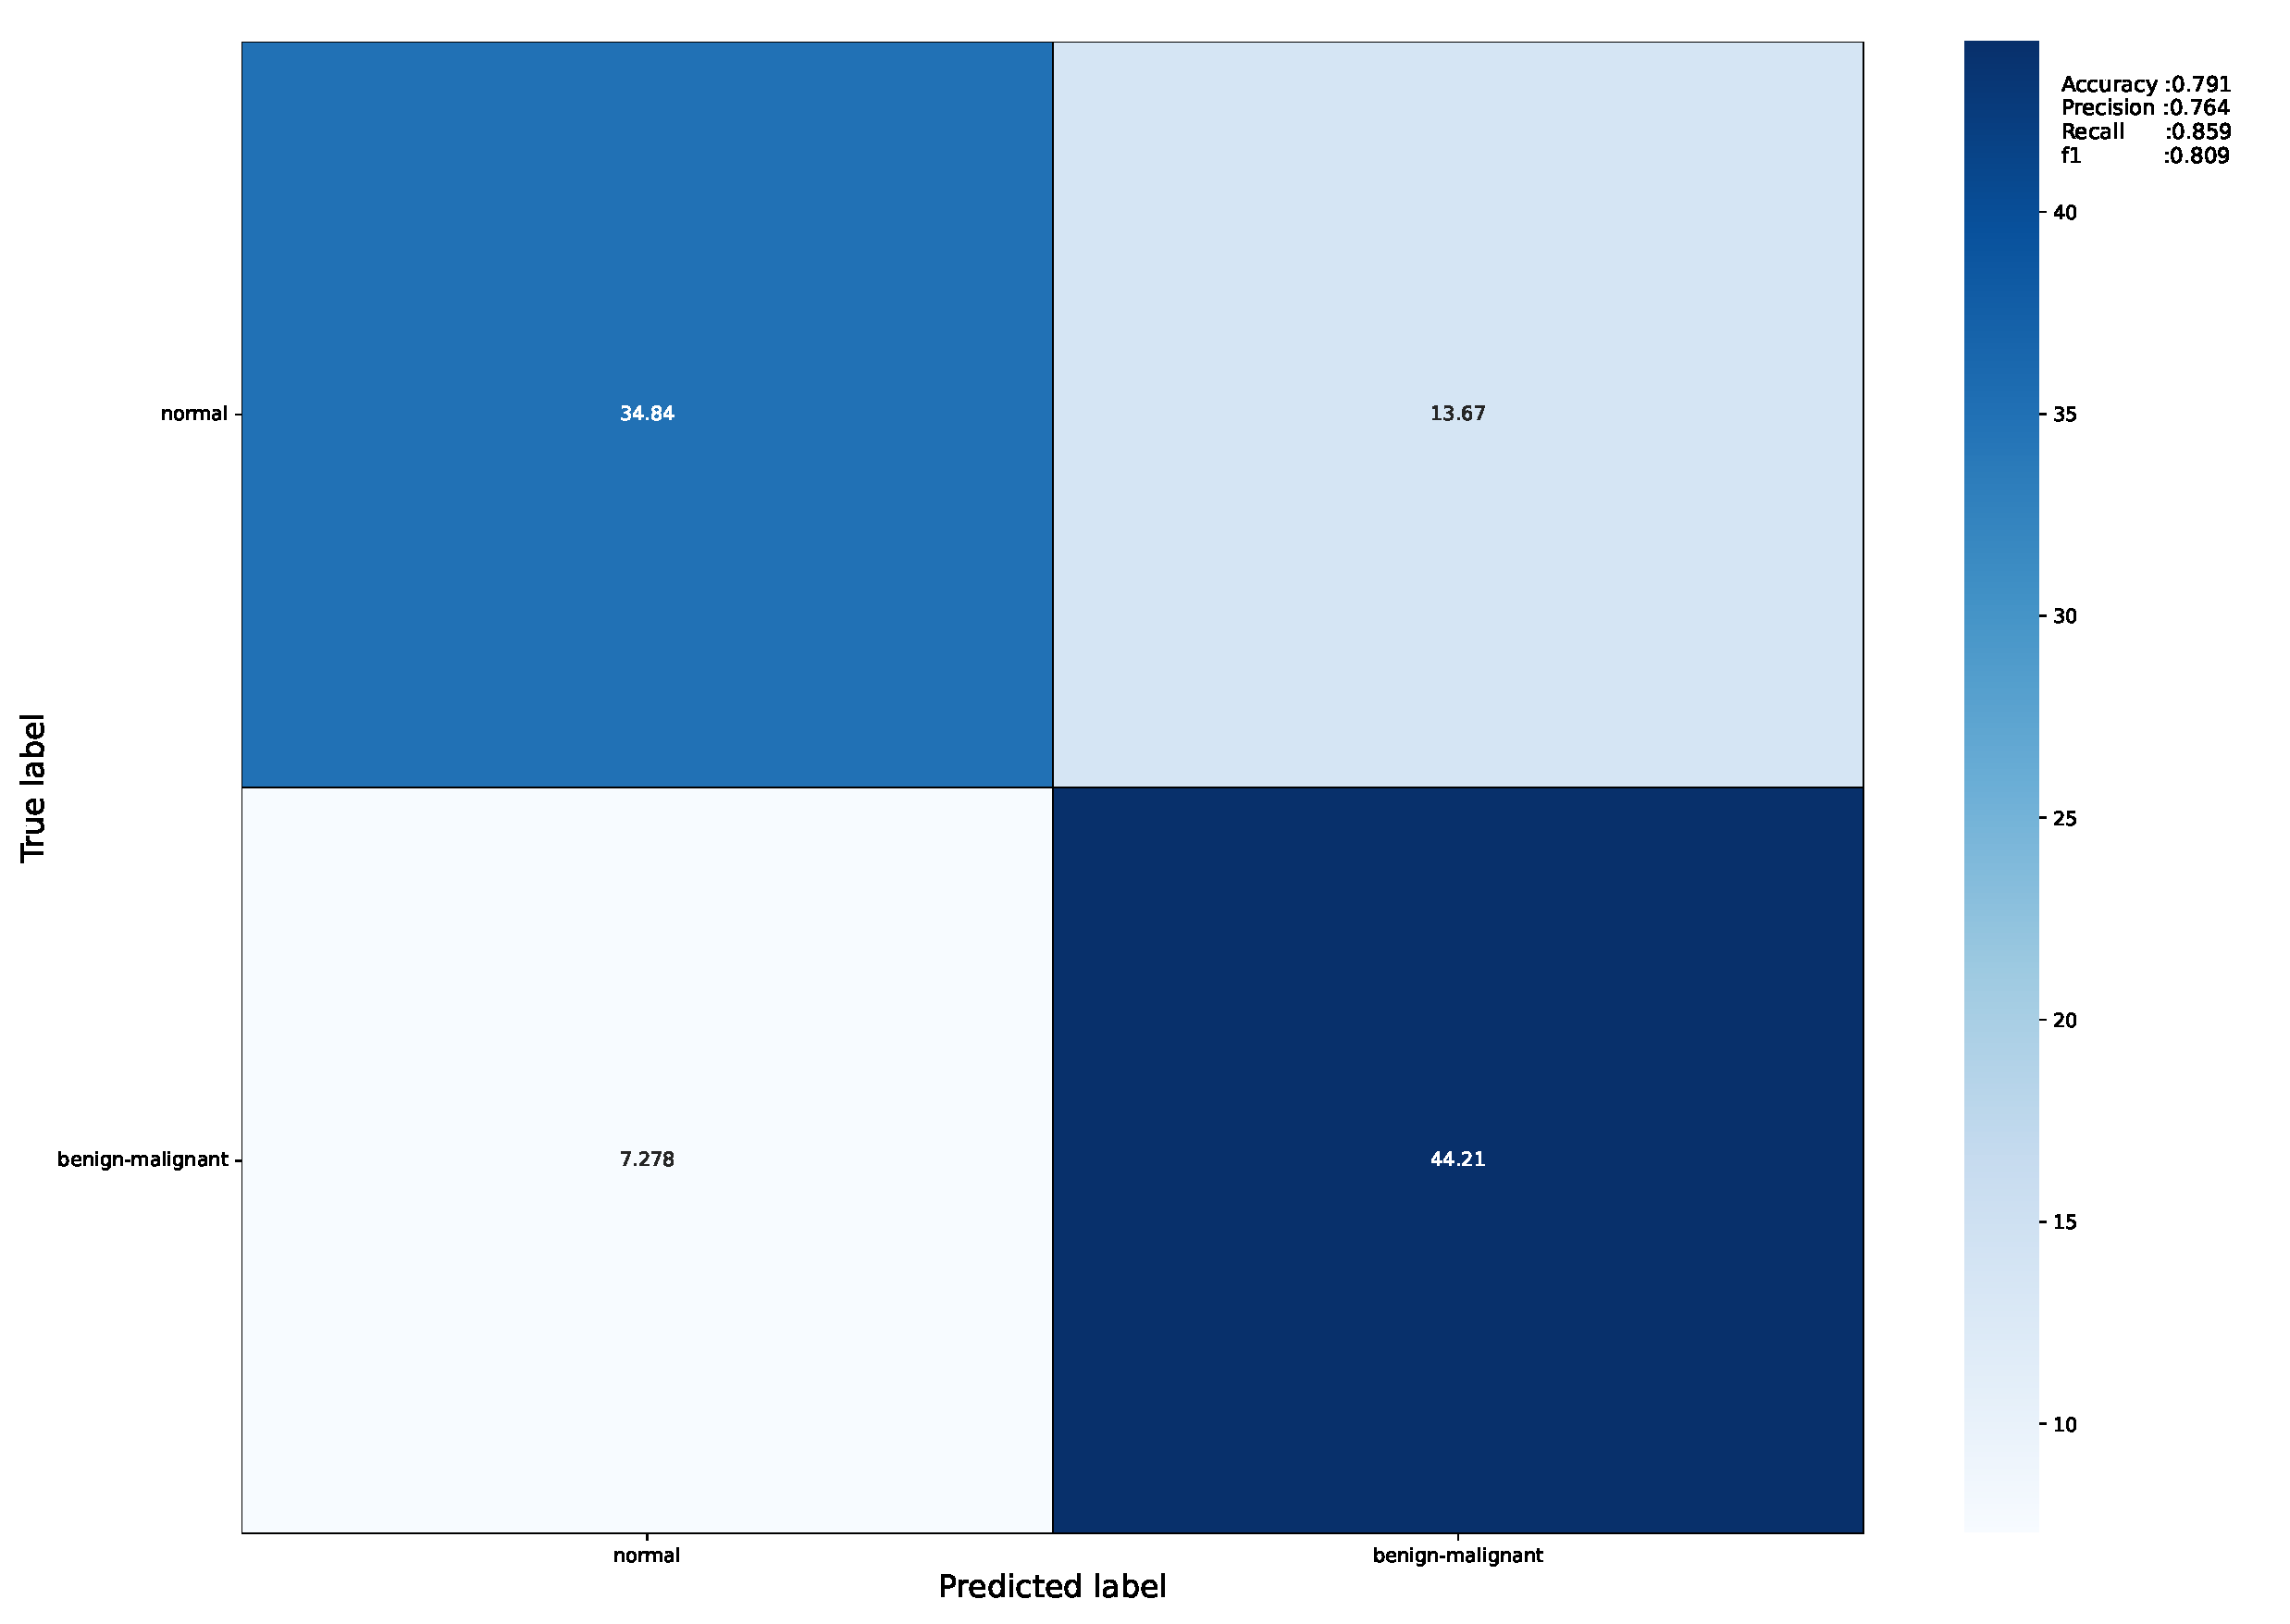
\includegraphics[width=\linewidth]{Figures/Confusion_Matrix_ML_Segmentation.pdf}
  \caption{Confusion matrix of traditional Machine Learning Segmentation task.}
  \label{Figure - ML_Segmentation Confusion matrix}
\end{figure}
The overall accuracy of the model was determined to be $79.06\%$, indicating that it achieved a high level of overall correctness in its predictions.

For the tumour class, the precision was calculated as $82.72\%$, indicating that approximately $82.72\%$ of the predicted tumour instances were accurate. For the non-tumour class, the precision was $76.38\%$, signifying that around $76.38\%$ of the predicted non-tumour instances were correct.

The recall values differed for the two classes. The tumour class displayed a recall of $71.83\%$, indicating that only about $71.83\%$ of the actual tumour instances were correctly identified. In contrast, the non-tumour class exhibited a higher recall of $85.86\%$, reflecting a more accurate identification of non-tumour instances.

The F1 score for the tumour class was calculated as $76.89\%$, taking into account both precision and recall for this class. Similarly, the F1 score for the non-tumour class was $80.85\%$, representing the harmonic mean of precision and recall for this class.

In summary, the final model achieved an overall accuracy of $79.06\%$ and demonstrated varying levels of precision, recall, and F1 score for each class. These metrics provide valuable insights into the model's performance in correctly classifying tumour and non-tumour instances. It is important to note that the baseline accuracy for this task was $48.45\%$.

In Figures \ref{Figure - ML_Segmentation First case of Image Segmentation} and \ref{Figure - ML_Segmentation Second case of Image Segmentation}, we showcase the outcomes of the segmentation algorithm when applied to two distinct cases.
	\begin{figure}
  		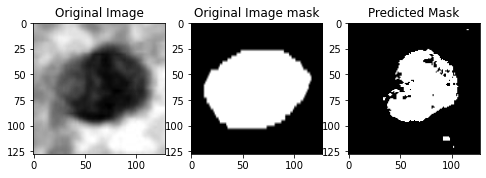
\includegraphics[width=\linewidth]{Figures/segment_ml_1.png}  		  				
  		\caption{First case of Image Segmentation for Machine Learning model.}
		\label{Figure - ML_Segmentation First case of Image Segmentation}
  	\end{figure}
  	\begin{figure}
  		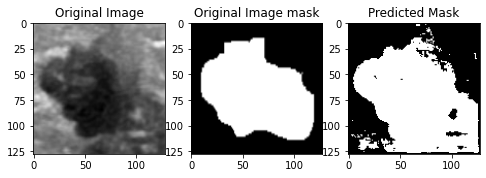
\includegraphics[width=\linewidth]{Figures/segment_ml_2.png}  		  				
  		\caption{Second case of Image Segmentation for Machine Learning model.}
		\label{Figure - ML_Segmentation Second case of Image Segmentation}
  	\end{figure}

%%%%%%%%%%%%%%%%%%%%%%%%%%%%%%%%%%%%%%%%%%%%%%%%%%%%%%%%%%%%%%%%%%%%%%%%%%%
%%%%%%%%%%%%%%%%%%%%%%%%%%%%%%%%%%%%%%%%%%%%%%%%%%%%%%%%%%%%%%%%%%%%%%%%%%%
%%%%%%%%%%%%%%%%%%%%%%%%%%%%%%%%%%%%%%%%%%%%%%%%%%%%%%%%%%%%%%%%%%%%%%%%%%%
%%%%%%%%%%%%%%%%%%%%%%%%%%%%%%%%%%%%%%%%%%%%%%%%%%%%%%%%%%%%%%%%%%%%%%%%%%%
%%%%%%%%%%%%%%%%%%%%%%%%%%%%%%%%%%%%%%%%%%%%%%%%%%%%%%%%%%%%%%%%%%%%%%%%%%%
%%%%%%%%%%%%%%%%%%%%%%%%%%%%%%%%%%%%%%%%%%%%%%%%%%%%%%%%%%%%%%%%%%%%%%%%%%%
%%%%%%%%%%%%%%%%%%%%%%%%%%%%%%%%%%%%%%%%%%%%%%%%%%%%%%%%%%%%%%%%%%%%%%%%%%%
%%%%%%%%%%%%%%%%%%%%%%%%%%%%%%%%%%%%%%%%%%%%%%%%%%%%%%%%%%%%%%%%%%%%%%%%%%%

\section{Image Classification Using Deep Learning Algorithms}

\subsection{Description}
In this section, our focus is on utilizing deep learning techniques to address our classification problem. Due to the limited number of available images (approximately 800), training a new convolutional neural network (CNN) from scratch would be challenging. Therefore, we employ the transfer learning approach. With transfer learning, we can leverage the knowledge and pre-trained weights of existing CNN architectures. While several architectures were suitable for our task, we opted to utilize VGG19 and its pre-trained weights from the ImageNet dataset.

\subsection{Data Preprocessing}
In order to utilize the VGG19 model, some adjustments were necessary. Firstly, we resized our images to match the required dimensions of (224, 224). This ensured compatibility with the model's input size. Additionally, the VGG19 architecture is primarily designed to handle RGB images, which consist of three color channels. However, our ultrasound images are originally grayscale. To address this, we converted the grayscale images to RGB format. It is important to note that this conversion does not introduce actual colors to the images rather, it involves replicating the grayscale channel across all three channels to match the expected input format of VGG19. This modification allowed us to effectively employ the VGG19 model for our classification task.

In addition to the aforementioned modifications, we performed data augmentation on the training set, which initially consisted of $80\%$ of the total dataset. Recognizing that approximately 650 images might not provide sufficient training data, we opted to augment the dataset by generating rotated versions of the images at 45-degree increments. When comparing the results between the augmented and non-augmented cases, we observed no significant difference in performance. Nonetheless, we chose to retain the augmented data as it contributes to a more comprehensive and robust training pipeline.

\subsection{Model}
As mentioned earlier, we implemented transfer learning using the VGG19 model. To adapt the model to our task, we kept all but the last two layers frozen, as we had a limited number of images. Additionally, we introduced two extra layers. The first layer is a dense layer with 50 neurons and a ReLU activation function. This intermediate layer serves as a bridge between the flattened output of the VGG19 model and the subsequent layers. Its purpose is to extract higher-level features and capture more abstract representations from the input data.

The second additional layer is another dense layer with 20 neurons, also employing the ReLU activation function. This layer further refines the learned representations, allowing the model to capture finer details and intricacies in the data.

Finally, we appended a prediction layer with the softmax activation function. This layer produces the final output probabilities for each class. By using softmax, the model's predictions are transformed into a probability distribution, providing insights into the model's confidence in its classifications.

During the training procedure, we employ 15 epochs with the Adam optimizer. Categorical cross-entropy is used as the loss function, which is suitable for multi-class classification tasks. The goal is to minimize the discrepancy between the predicted class probabilities and the true class labels. Additionally, we track the accuracy metric to assess the model's performance and convergence. This metric measures the proportion of correctly classified samples. By utilizing this setup, we aim to optimize the model's performance on the classification task.

Once the training of our model is complete, we take the necessary steps to save it. This enables us to reuse the model without having to train it from the beginning every time.

\subsection{Results}
We evaluated the performance of the classifier on the test set and the results are presented in the following Table \ref{Table - DL_Classification Test accuracy-precision-recall-f1 results for our model}
\begin{table}[H]
\centering
\begin{tabular}{cc}
Accuracy  & 0.796               \\
Precision & 0.71, 0.857, 0.738  \\
Recall    & 0.815, 0.818, 0.738 \\
F1 score  & 0.759, 0.837, 0.738
\end{tabular}
\caption{The metrics for the test set using the trained model. Precision, Recall, and F1 score are provided for each class separately, with the classes being normal, benign, and malignant.}
\label{Table - DL_Classification Test accuracy-precision-recall-f1 results for our model}
\end{table}
If we compare the results of our deep learning model with the results presented in Table \ref{Table - ML_Classification Test accuracy-precision-recall-f1 results for voting classifier}, we can clearly observe that our deep learning approach provides significantly better outcomes. The deep learning model demonstrates higher accuracy, precision, recall, and F1 scores, indicating its superior performance in classifying tumours in the breast ultrasound images. These improved results affirm the effectiveness of our deep learning methodology in achieving more accurate and reliable predictions compared to the previous traditional machine learning approach.

We also provide the confusion matrix of our problem in Figure \ref{Figure - DL_Classification Confusion matrix}.
\begin{figure}
  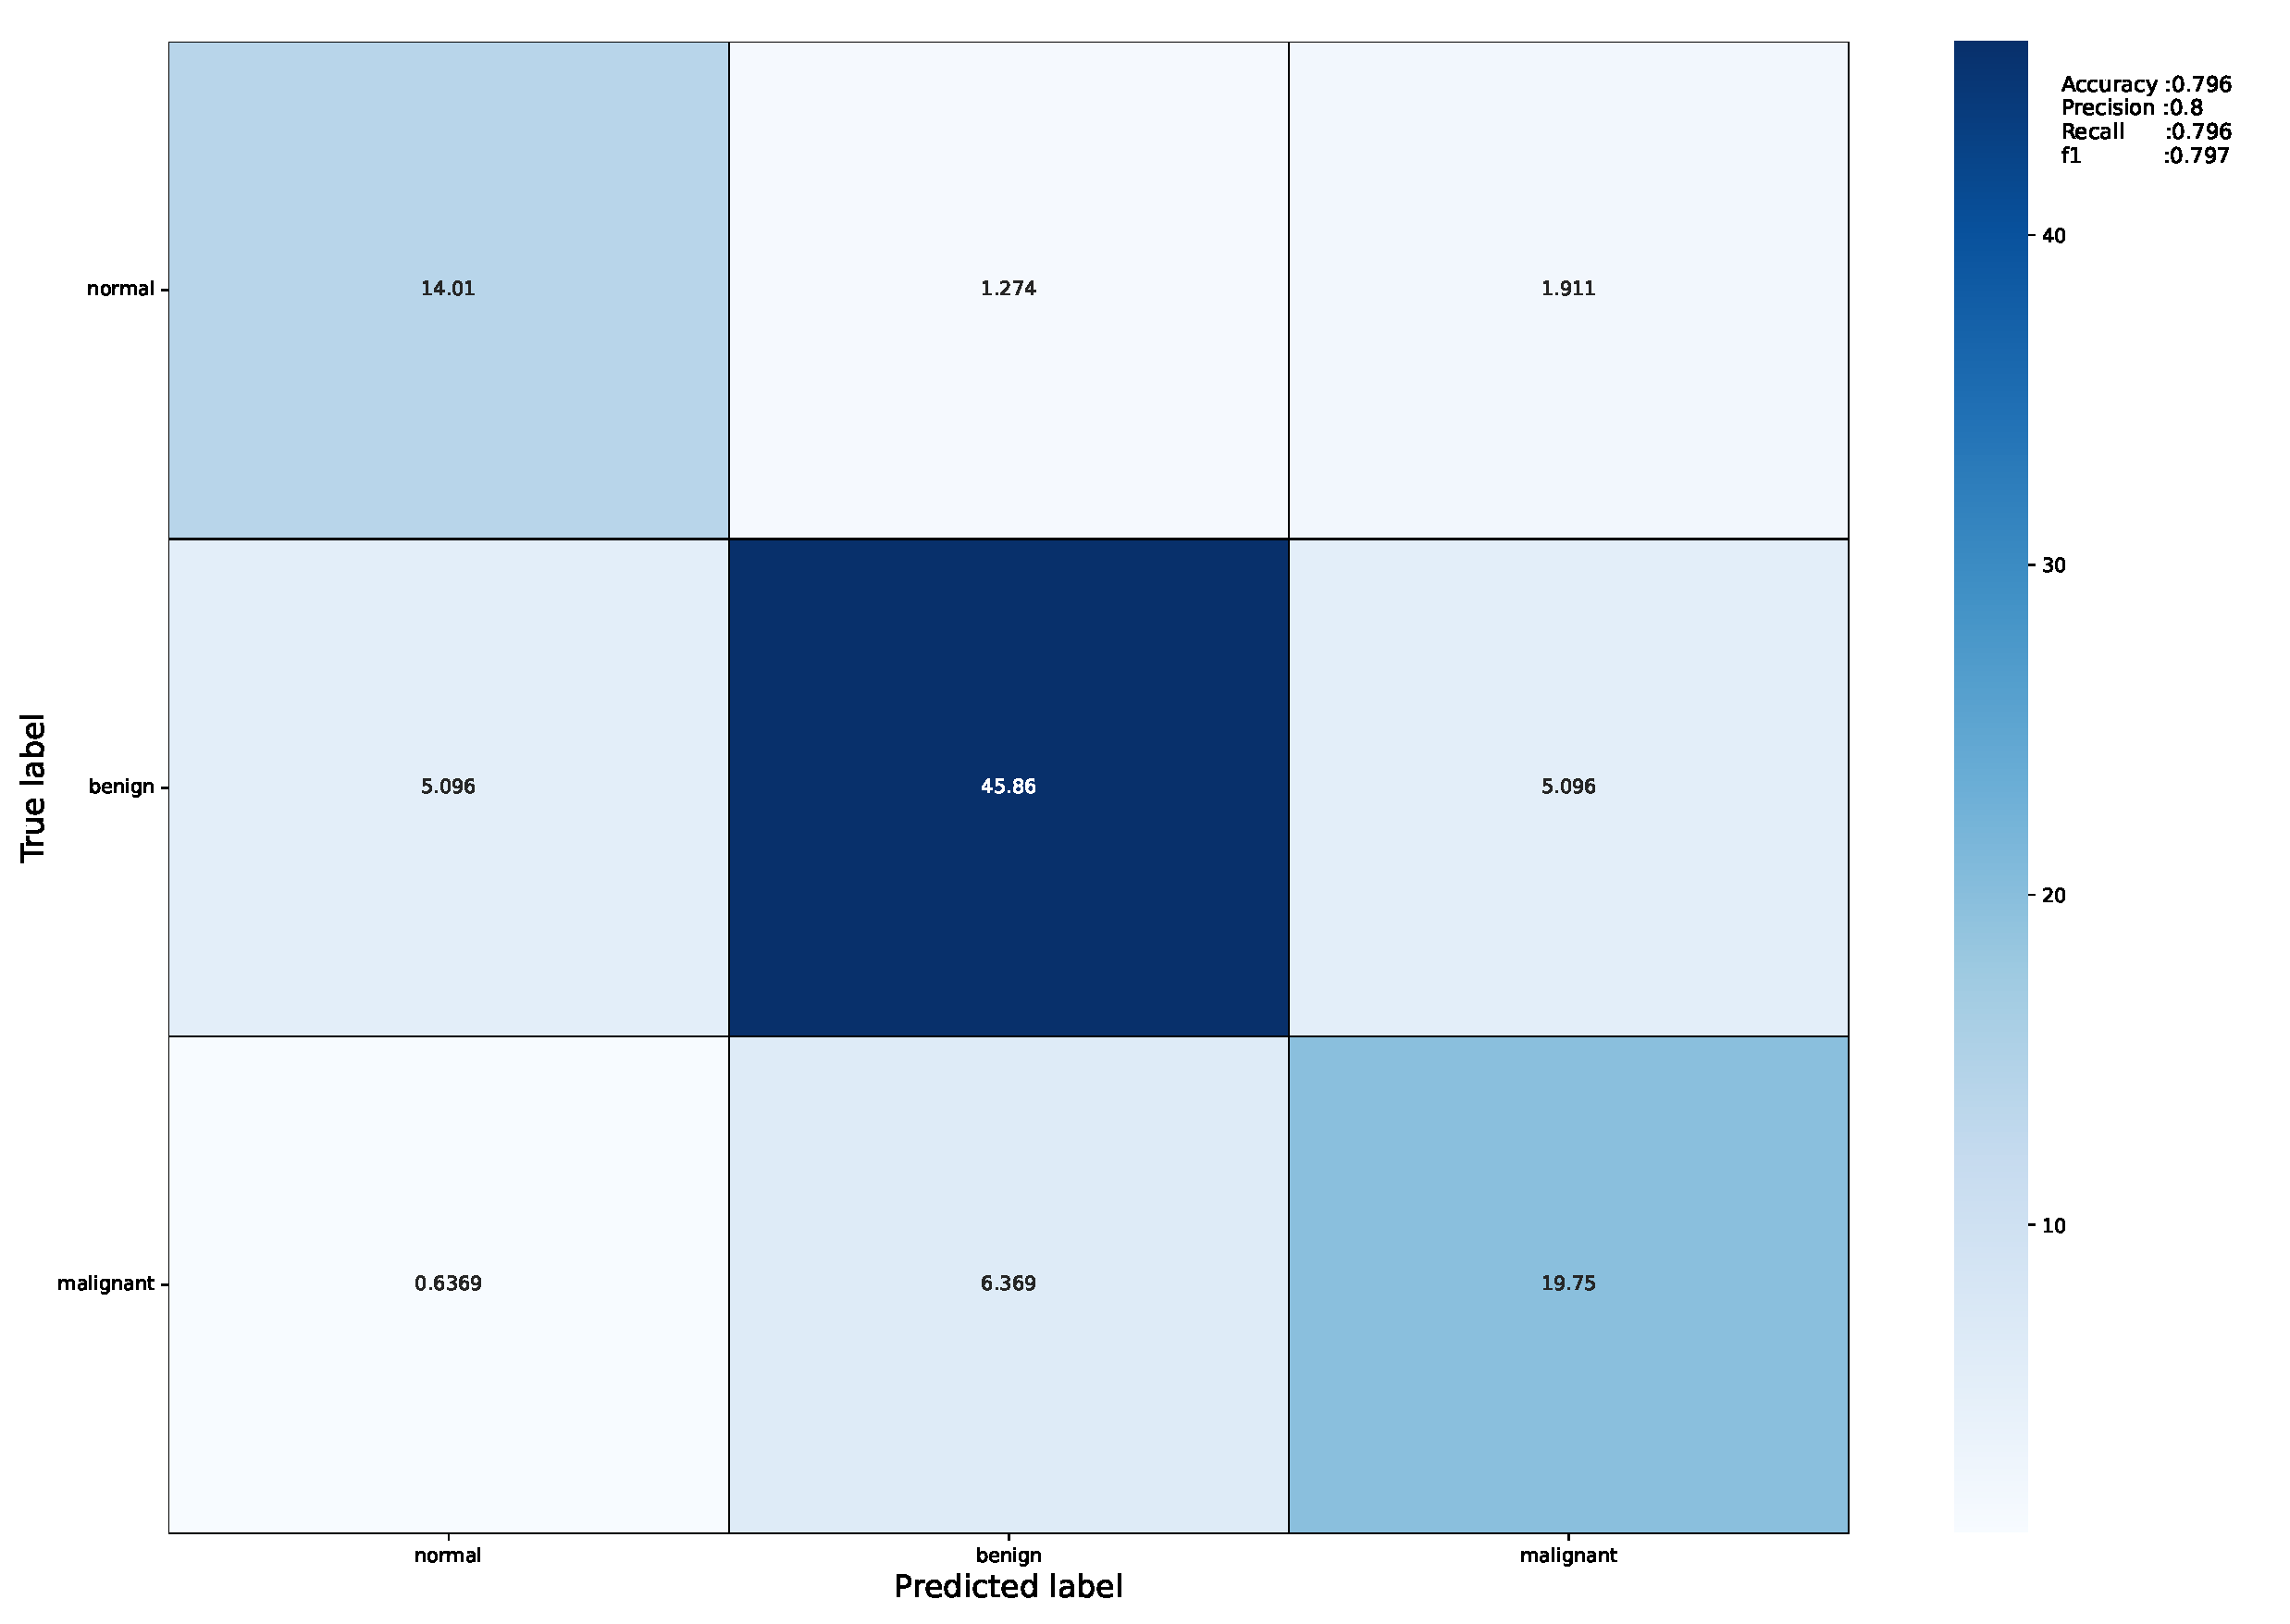
\includegraphics[width=\linewidth]{Figures/Confusion_Matrix_DL_Classification.pdf}
  \caption{Confusion matrix of Deep Learning Classification task.}
  \label{Figure - DL_Classification Confusion matrix}
\end{figure}

For a better understanding of the effectiveness of our models, we also provide the baseline accuracy. The baseline accuracy serves as a reference point to evaluate the performance of our classification models. In this task, the baseline accuracy was determined to be $56.03\%$. By comparing the accuracy of our models with the baseline accuracy, we can assess the improvement achieved by our approach. 

%%%%%%%%%%%%%%%%%%%%%%%%%%%%%%%%%%%%%%%%%%%%%%%%%%%%%%%%%%%%%%%%%%%%%%%%%%%
%%%%%%%%%%%%%%%%%%%%%%%%%%%%%%%%%%%%%%%%%%%%%%%%%%%%%%%%%%%%%%%%%%%%%%%%%%%
%%%%%%%%%%%%%%%%%%%%%%%%%%%%%%%%%%%%%%%%%%%%%%%%%%%%%%%%%%%%%%%%%%%%%%%%%%%
%%%%%%%%%%%%%%%%%%%%%%%%%%%%%%%%%%%%%%%%%%%%%%%%%%%%%%%%%%%%%%%%%%%%%%%%%%%
%%%%%%%%%%%%%%%%%%%%%%%%%%%%%%%%%%%%%%%%%%%%%%%%%%%%%%%%%%%%%%%%%%%%%%%%%%%
%%%%%%%%%%%%%%%%%%%%%%%%%%%%%%%%%%%%%%%%%%%%%%%%%%%%%%%%%%%%%%%%%%%%%%%%%%%
%%%%%%%%%%%%%%%%%%%%%%%%%%%%%%%%%%%%%%%%%%%%%%%%%%%%%%%%%%%%%%%%%%%%%%%%%%%
%%%%%%%%%%%%%%%%%%%%%%%%%%%%%%%%%%%%%%%%%%%%%%%%%%%%%%%%%%%%%%%%%%%%%%%%%%%

\section{Image Segmentation Using Deep Learning Algorithms}

\subsection{Description}
In this section, we focus on the segmentation task using Deep Learning architecture. As observed in the previous section, traditional machine learning methods face several limitations when applied to segmentation tasks. Notably, we had to rely on cropping around the tumour region to achieve satisfactory segmentation. However, this approach assumes prior knowledge of the tumour's location, which is not a practical assumption. Moreover, even with this assumption, the obtained results were not optimal. Therefore, based on our findings, we can conclude that machine learning techniques are not well-suited for this particular segmentation task. 

For our solution, we once again relied on the VGG19 model and utilized its pre-trained weights from ImageNet. As described earlier, this architecture served as the foundation for our approach. 

Lastly, it is important to note that we approached the problem as a binary classification task, focusing solely on identifying the cancerous areas without distinguishing between benign and malignant tumours. Our goal was to locate and segment the regions of interest associated with cancerous tissue, regardless of its specific nature.

\subsection{Data Preprocessing}
The preprocessing pipeline for the segmentation task follows a similar approach to the classification task, with a few notable differences. While we won't delve into a detailed analysis of the pipeline, we will highlight the key distinctions. Firstly, no data augmentation was applied in this case and secondly, as we are working with the tumour masks, we also resized the mask images to ensure compatibility with the model.

\subsection{Model}
For this particular task, we decided to freeze all the layers of the VGG19 model and instead focus on building the decoder part. The decoder architecture we used in our model was heavily influenced by a previous research paper, which served as a reference for designing this component \cite{decoder}.

\subsection{Results}
In this task, we purposely avoided applying any cropping to our images, which means we anticipate having a heavily imbalanced dataset. It's important to note that in this context, our focus is on individual pixels, essentially performing pixel-level image classification. As one would expect, the majority of pixels in the images correspond to non-cancerous regions, while only a small portion is associated with tumorous areas.

The baseline accuracy that we calculated for this task is approximately $92.06\%$. Therefore, in order to consider our algorithm effective, we need to surpass this baseline accuracy and achieve higher performance.

After applying the trained model to our test set, we get the following results:
\begin{table}[H]
\centering
\begin{tabular}{cc}
Accuracy  & 0.957        \\
Precision & 0.973 0.721 \\
Recall    & 0.98 0.651 \\
F1 score  & 0.977 0.684
\end{tabular}
\caption{The performance metrics of the model on the test set are presented below. Precision, recall, and F1 score are reported for both the tumour and non-tumour classes.}
\label{Table - DL_Segmentation Test accuracy-precision-recall-f1 results for model}
\end{table}

The confusion matrix for the test set is presented in Figure \ref{Figure - DL_Segmentation Confusion matrix}.
\begin{figure}
  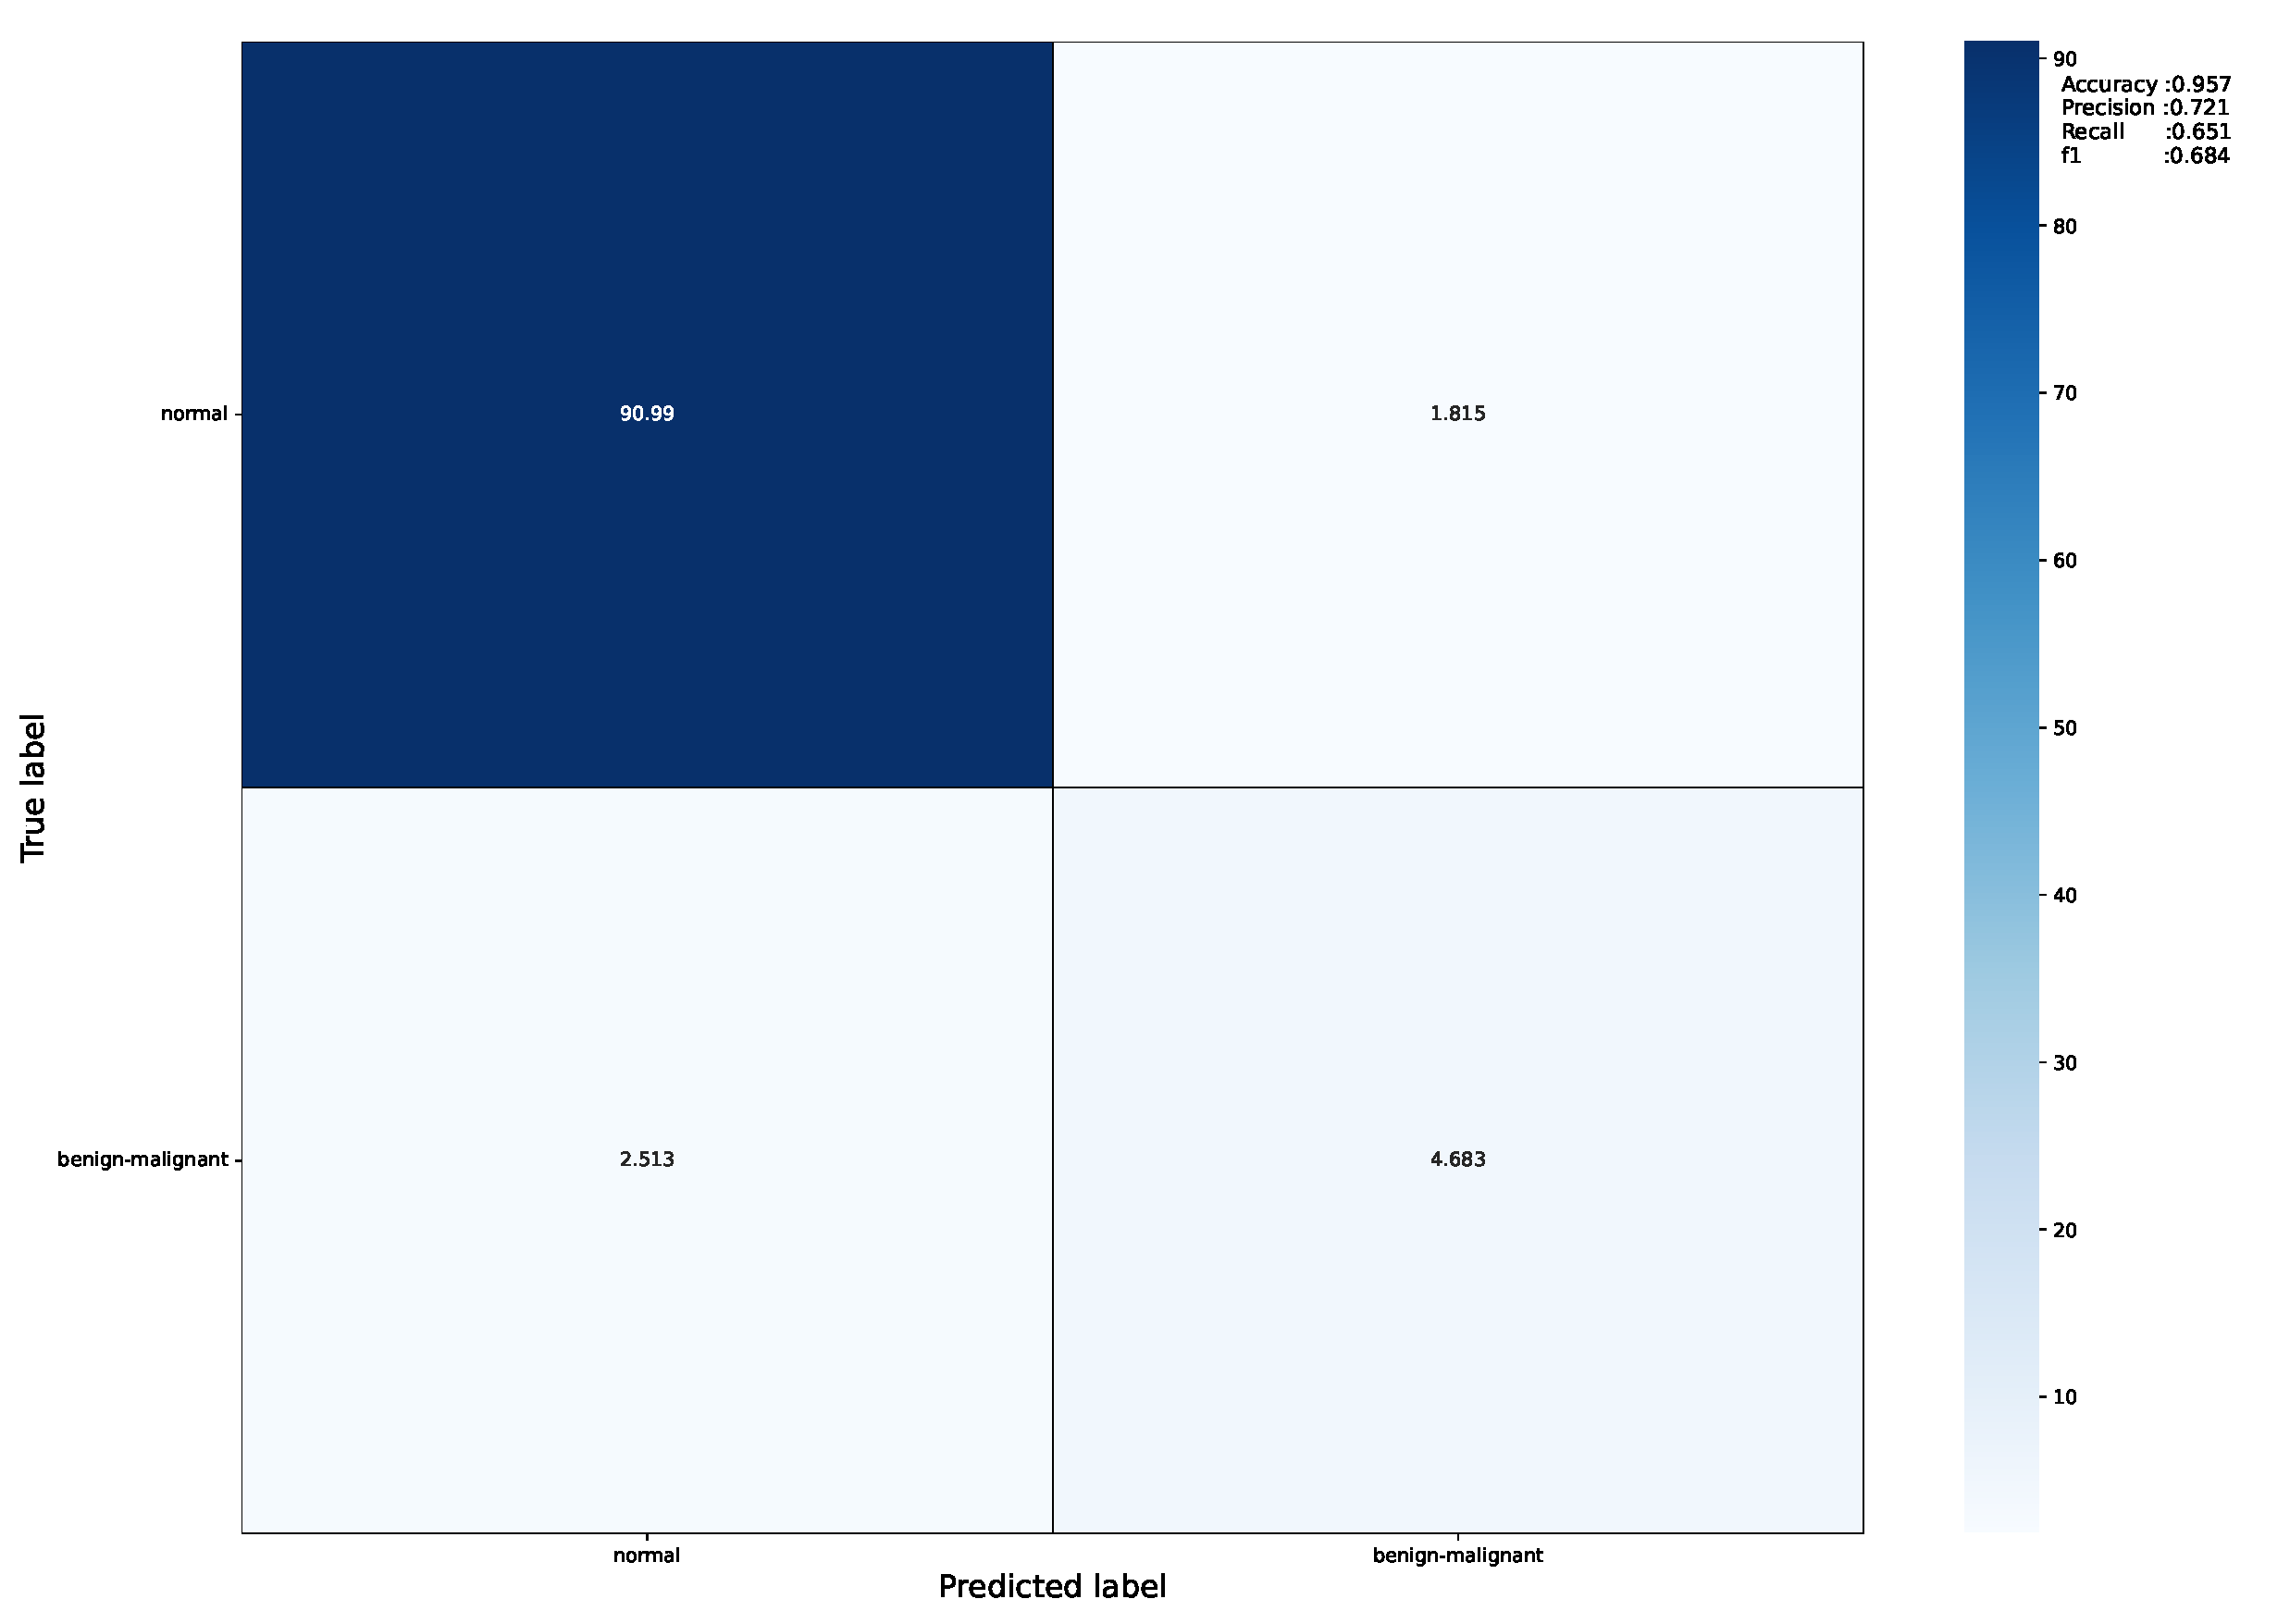
\includegraphics[width=\linewidth]{Figures/Confusion_Matrix_DL_Segmentation.pdf}
  \caption{Confusion matrix of Deep Learning Segmentation task.}
  \label{Figure - DL_Segmentation Confusion matrix}
\end{figure}

In a real-case scenario, we applied our algorithm to some ultrasound images and obtained the segmented tumours. The algorithm effectively processed the input images and produced segmentation masks highlighting the tumour regions. We present the results for three ultrasound images in Figures \ref{Figure - DL_Segmentation First case of Image Segmentation}-\ref{Figure - DL_Segmentation Third case of Image Segmentation}.
	\begin{figure}
  		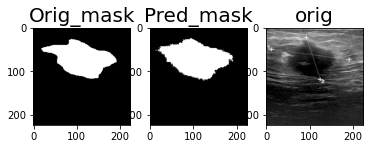
\includegraphics[width=\linewidth]{Figures/segment_dl_1.png}  		  							
  		\caption{First case of Image Segmentation for Deep Learning model.}
		\label{Figure - DL_Segmentation First case of Image Segmentation}
  	\end{figure}
  	\begin{figure}
  		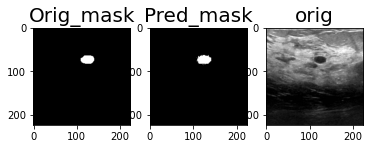
\includegraphics[width=\linewidth]{Figures/segment_dl_2.png}  		  							
  		\caption{Second case of Image Segmentation for Deep Learning model.}
		\label{Figure - DL_Segmentation Second case of Image Segmentation}
  	\end{figure}
  	\begin{figure}
  		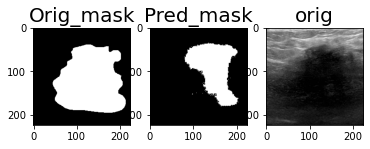
\includegraphics[width=\linewidth]{Figures/segment_dl_3.png}  		  							
  		\caption{Third case of Image Segmentation for Deep Learning model.}
		\label{Figure - DL_Segmentation Third case of Image Segmentation}
  	\end{figure}
From the analysis of Figures \ref{Figure - DL_Segmentation First case of Image Segmentation}-\ref{Figure - DL_Segmentation Third case of Image Segmentation}, we can observe that the tumour segmentation was highly accurate for the first two cases. However, in the third case, the segmentation results were not as satisfactory.

\subsection{Explainability Analysis}
The final analysis conducted for the deep learning segmentation task was the explainability analysis. The objective was to gain a deeper understanding of the areas within the images that the neural network considers crucial for the segmentation process. By examining the Figures, specifically Figures \ref{Figure - DL_Segmentation explainability First case of Image Segmentation} to \ref{Figure - DL_Segmentation explainability Third case of Image Segmentation}, it becomes apparent that the regions surrounding and containing the tumours play a pivotal role in the segmentation task.
	\begin{figure}
  		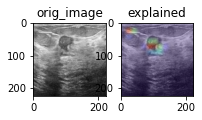
\includegraphics[width=\linewidth]{Figures/segment_explained_dl_1.png}
  		\caption{First case of explainability in Image Segmentation for Deep Learning model.}
		\label{Figure - DL_Segmentation explainability First case of Image Segmentation}
  	\end{figure}
  	\begin{figure}
  		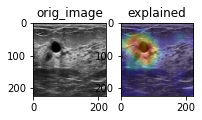
\includegraphics[width=\linewidth]{Figures/segment_explained_dl_2.png}
  		\caption{Second case of explainability in Image Segmentation for Deep Learning model.}
		\label{Figure - DL_Segmentation explainability Second case of Image Segmentation}
  	\end{figure}
  	\begin{figure}
  		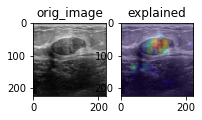
\includegraphics[width=\linewidth]{Figures/segment_explained_dl_3.png}
  		\caption{Third case of explainability in Image Segmentation for Deep Learning model.}
		\label{Figure - DL_Segmentation explainability Third case of Image Segmentation}
  	\end{figure}

%%%%%%%%%%%%%%%%%%%%%%%%%%%%%%%%%%%%%%%%%%%%%%%%%%%%%%%%%%%%%%%%%%%%%%%%%%%
%%%%%%%%%%%%%%%%%%%%%%%%%%%%%%%%%%%%%%%%%%%%%%%%%%%%%%%%%%%%%%%%%%%%%%%%%%%
%%%%%%%%%%%%%%%%%%%%%%%%%%%%%%%%%%%%%%%%%%%%%%%%%%%%%%%%%%%%%%%%%%%%%%%%%%%
%%%%%%%%%%%%%%%%%%%%%%%%%%%%%%%%%%%%%%%%%%%%%%%%%%%%%%%%%%%%%%%%%%%%%%%%%%%
%%%%%%%%%%%%%%%%%%%%%%%%%%%%%%%%%%%%%%%%%%%%%%%%%%%%%%%%%%%%%%%%%%%%%%%%%%%
%%%%%%%%%%%%%%%%%%%%%%%%%%%%%%%%%%%%%%%%%%%%%%%%%%%%%%%%%%%%%%%%%%%%%%%%%%%
%%%%%%%%%%%%%%%%%%%%%%%%%%%%%%%%%%%%%%%%%%%%%%%%%%%%%%%%%%%%%%%%%%%%%%%%%%%
%%%%%%%%%%%%%%%%%%%%%%%%%%%%%%%%%%%%%%%%%%%%%%%%%%%%%%%%%%%%%%%%%%%%%%%%%%%

\section{Conclusion}
In this task, we explored two distinct topics: image classification and image segmentation, employing both traditional machine learning and deep learning methodologies. Our primary objective was to evaluate the capabilities and limitations of each approach and compare their performance. Additionally, we conducted an explainability analysis to identify the influential areas within the images as determined by our neural networks.

In the traditional machine learning approach, we achieved satisfactory results for the image classification task. However, the image segmentation task presented several challenges. The algorithm exhibited difficulties in distinguishing between the dark areas of the tumours and the surrounding margin regions. Consequently, we resorted to manually cropping the images around the tumours during both the training and testing phases. While this approach may be acceptable for the training set, it becomes impractical for the test set as it assumes prior knowledge of the tumour location.

On the other hand, the application of deep learning techniques proved to be more efficient and yielded superior results. For both the classification and segmentation tasks, we leveraged transfer learning techniques by utilizing the pre-trained VGG19 model. The segmentation task, in particular, demonstrated significant improvements, successfully localizing tumour regions in many cases. Our explainability analysis further validated the significance of these regions, confirming that areas belonging to or surrounding the tumour played a pivotal role in our segmentation task.

Overall, deep learning techniques outperformed traditional machine learning approaches in terms of ease of implementation and achieved better results. The utilization of transfer learning with the VGG19 model significantly enhanced the performance of both classification and segmentation tasks. These findings underscore the potential of deep learning in medical imaging, with implications for improved tumour detection and localization.

\section{Future Work}
Here are several potential areas for future work:
\begin{itemize}
\item Further investigation into additional data augmentation techniques and a comparative analysis with the findings of the present study should be considered..
\item Exploration of additional data augmentation techniques, followed by a comparison of the results obtained with those reported in the current paper.
\item Combining multiple models or predictions through ensemble learning techniques could be explored to further improve the accuracy and robustness of the classification and segmentation results.
\end{itemize}

\begin{thebibliography}{00}
\bibitem{dataset} https://www.kaggle.com/datasets/aryashah2k/breast-ultrasound-images-dataset
\bibitem{decoder} "U-Net: Convolutional Networks for Biomedical Image Segmentation" by Olaf Ronneberger, Philipp Fischer, and Thomas Brox, 2015
\end{thebibliography}
\vspace{12pt}
\color{red}